\chapter{\IfLanguageName{dutch}{Stand van zaken}{State of the art}}
\label{ch:stand-van-zaken}

% Tip: Begin elk hoofdstuk met een paragraaf inleiding die beschrijft hoe
% dit hoofdstuk past binnen het geheel van de bachelorproef. Geef in het
% bijzonder aan wat de link is met het vorige en volgende hoofdstuk.

% Pas na deze inleidende paragraaf komt de eerste sectiehoofding.
\subsection{Software release management for component-based software}
Een van de eerste vragen die opdook was: “Hoe wordt software release management nu eigenlijk verwezenlijkt?”. Zijn er bepaalde procedures of praktijken die gevolgd worden om dit in goed banen te lijden. Welke technieken worden er gevolgd? Dit leidde ertoe om in de eerste plaats in de richting van de ITIL-processen te zoeken (ITIL, Information Technology Infrastructure Library). Dit omdat het nauw aansluit bij software release management. De volgende paper \autocite{Hoek2002} is een resultaat van de papers bij de zoek term ‘ITIL’.
\newline
\newline
De paper \autocite{Hoek2002} is een rapport, verslag over een jarenlange observatie van software release management praktijken. Deze paper \autocite{Hoek2002} is niet meer van de jongste maar bespreekt toch nog een aantal belangrijke kernideeën. De technische kant en de gebruikte software is minder relevant.
\newline
\newline
De paper \autocite{Hoek2002} begint met de problematiek uit te leggen van software release management voor zowel de gebruiker als de ontwikkelaar. In de eerste plaats stelt de paper dat de eindgebruiker altijd het slachtoffer is. Tegenwoordig wordt er veel component gebaseerde software ontwikkelt. Een goed voorbeeld hiervan, zijn Linux packages. Dit maakt het niet altijd gemakkelijk voor de eindgebruiker om de juiste softwarecomponenten te vinden. Laat staan dat het de juiste versies zijn. Voeg daar dan nog aan toe dat sommige softwarebedrijven niet altijd oudere versies aanbieden, dat de eindgebruiker meerdere websites moet afsporen en dat de eindgebruiker ook nog eens verantwoordelijk is voor het installeren en up-to-date houden van al die componenten. Dit is dus ver van een optimale situatie.
\newline
\newline
Het samenvoegen van verschillende componenten, het uitrollen naar de gebruikers en het updaten ervan, wordt beschreven als software release management. Software release management is enkel verantwoordelijk voor het beheren en het opslaan van de verschillende benodigde componenten en is dus niet bedoelt om de verschillende componenten zelf te compileren of afleiden. Dit zorgt ervoor dat software release management tools compleet platform onafhankelijk kunnen zijn. Het limiteert daardoor wel de functionaliteit. In het bijzonder is de tool niet instaat om aan validatie of versie beheer te doen.
\newline
\newline
Om aan goede software release management te kunnen doen, is goede documentatie van alle verschillende componenten nodig. De paper stelt een aantal vereisten voor software release management voor. Dit is voor zowel de eindgebruiker als de ontwikkelaar. Deze hebben ze samengesteld uit hun eigen tien jaar lange ervaring. \autocite{Hoek2002}.
\newline
\newline
\textbf{Minimale vereisten voor ontwikkelaars:}
\begin{itemize}
    \item Afhankelijkheden moeten expliciet zijn en gemakkelijk kunnen worden vastgelegd.
    \item Releases moeten consistent worden gehouden.
    \item De reikwijdte van een release moet controleerbaar zijn.
    \item Het releaseproces zou minimale inspanning aan de kant van de ontwikkelaar moeten inhouden.
    \item Er moet een geschiedenis van opvragen worden bijgehouden.
\end{itemize}
\textbf{Minimale vereisten voor eindgebruiker:}
\begin{itemize}
    \item Beschrijvende informatie moet beschikbaar zijn.
    \item Er moet transparantie over de locatie worden geboden.
    \item Een component en zijn afhankelijkheden moeten als één archief kunnen worden opgehaald.
    \item Software-implementatie hulpmiddelen moeten de software-releasebeheertool kunnen gebruiken als bron voor componenten die moeten worden geïnstalleerd en geconfigureerd.
\end{itemize}
Hierna geeft de paper \autocite{Hoek2002} verder uitleg over een software release management tool die de schrijvers van de paper zelf hebben ontwikkeld. Dit is minder interessant voor de doeleinden van dit onderzoek maar de ideeën achter deze tool kunnen een meerwaarde bieden bij de motivatie waarom software release management zo belangrijk is. 
\newline
\newline
De bedoeling van deze tool is om enerzijds de informatie die gebruikt wordt in het releasebeheer proces te structureren en anderzijds locatietransparantie aan te bieden.
\begin{figure}[H]
    \centering
    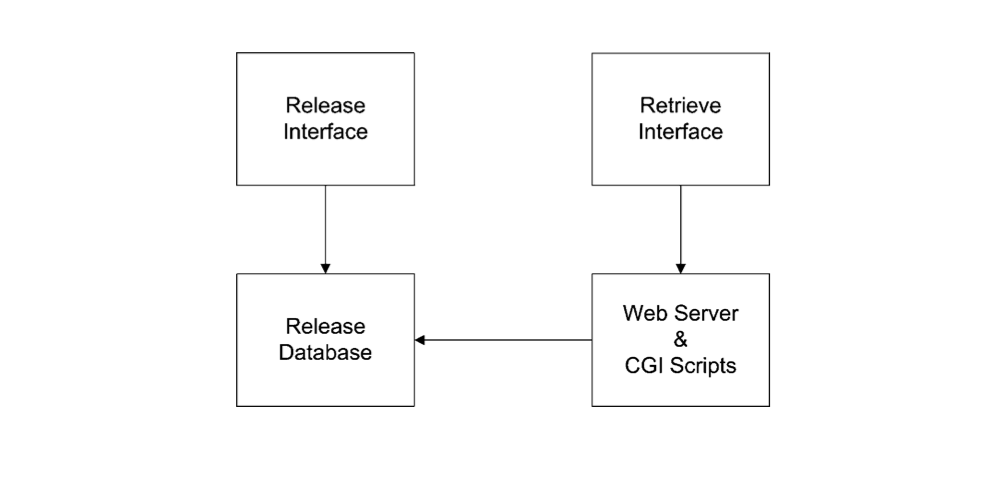
\includegraphics[width=\linewidth]{/Users/kenzie/Documents/HoGent/Bachelorproef/Images/SRM_Concept.png}
    \caption{Figuur uit \autocite{Hoek2002}. Figuur toont een simpele chart van hoe een software release management systeem opgebouwd kan zijn.}
    \label{fig:SRM_arch}
\end{figure}
De figuur~\ref{fig:SRM_arch} illustreert de architectuur van de software release management tool. Deze bestaat uit vier delen. Een logisch gecentraliseerde, maar fysiek gedistribueerde releasedatabase, een interface waarmee ontwikkelaars componenten in de releasedatabase plaatsen, een interface waarmee gebruikers componenten uit de releasedatabase halen en een webserver voor het op afstand toegang krijgen tot de releasedatabase en de componenten.
\newline
\newline
Deze paper \autocite{Hoek2002} stelt dus dat software release management ervoor moet zorgen dat componenten die op verschillende locaties, door verschillende bedrijven ontwikkeld worden, gemakkelijk gecentraliseerd toegankelijk moeten zijn. De bedrijven zelf hebben nog altijd volledige controle in handen van het versie beheer en het groeperen van de verschillende extern benodigde componenten. Tevens is de eindgebruiker nog altijd verantwoordelijk voor de installatie ervan maar dit begint ook minder het geval te zijn aangezien er meer en meer uitrol tools op de markt komen.
\newline
\newline
\subsection{Challenges and Problems in Release Management Process: A Case Study}
Zoals eerder aangehaald spelen ITIL-achtige procedures een belangrijke rol in software release management. Deze paper \autocite{Lahtela2011} is een korte casestudie met de bedoeling om kort een aantal problemen aan het licht te stellen in verband met software release binnen een bedrijf of organisatie naar een klant toe en hiervoor een oplossing aan te bieden.
\newline
\newline
De casestudie \autocite{Lahtela2011} beschrijft allereerst een definitie voor release management. “Release management omvat mensen, functies, systemen en activiteiten om software- en hardware versies effectief te plannen, verpakken, bouwen, testen en implementeren in een productie omgeving.”~\textcite{Lahtela2011} Deze definitie sluit goed aan bij wat we in dit onderzoek trachten te verduidelijken. Ook stelt de studie een redelijk belangrijk algemeen probleem. Helaas is in de praktijk bij veel bedrijven nog geen sprake van een implementatie van ITIL, ISO, enz. procedures. Dit omdat dit zeer moeilijk te implementeren is in reeds bestaande processen. Het hebben van zo een procedures is niet alleen zeer belangrijk om kwalitatief goede software op te leveren maar ook voor de supportafdeling van een bedrijf. Meestal zijn dit de mensen die het meeste te maken krijgen met deze procedures. Hierbij moet wel gezorgd worden dat er duidelijk verschil gemaakt wordt tussen het managen van veranderingen en het release management. Vervolgens beschrijft de studie de vastgestelde problemen en een mogelijk oplossing ervoor. Deze zijn letterlijk overgenomen uit de studie~\textcite{Lahtela2011}.
\begin{itemize}
    \item Er is geen gespecificeerd releasebeheerproces.
    \begin{itemize}
        \item Het releasebeheerproces moet worden beschreven en gestroomlijnd om ervoor te zorgen dat iedereen in de organisatie het proces kent.
    \end{itemize}
    \item De rol van releasemanager is onduidelijk.
    \begin{itemize}
        \item Iemand moet worden genoemd voor de rol van releasemanager. Daarnaast moeten de rollen, toewijzingen en verantwoordelijkheden worden beschreven.
    \end{itemize}
    \item De klant weet niet wat de release bevat.
    \begin{itemize}
        \item Meestal worden niet alle aangebrachte veranderingen beschreven of worden deze te technische beschreven waardoor de klant deze niet verstaat. De boodschap is om deze goed te documenteren op een verstaanbare manier.
    \end{itemize}
     \item De uitgifte distributie snelheid is te hoog.
    \begin{itemize}
        \item De release-vensters, die het tijdstip bepalen waarop de release in de productieomgeving van de klant moet worden geïnstalleerd, moeten worden overeengekomen tussen de serviceprovider en de klant, bijvoorbeeld grote releases maandelijks en kleinere releases wekelijks.
    \end{itemize}
    \item De klant denkt dat de serviceprovider niet alle testgevallen kan testen of inspecteren.
    \begin{itemize}
        \item Het testproces, dat deels wordt gedaan binnen het release managementproces, moet worden ontwikkeld. Het proces moet worden beschreven en aan producttesters worden geleerd. Daarnaast moeten de testresultaten aan de klant worden voorgelegd.
    \end{itemize}
    \item Er moeten meer testomgevingen in het testproces zijn.
    \begin{itemize}
        \item Er moet worden onderzocht of er meer testomgevingen nodig zijn. De ideale situatie is dat er voor elke productieomgeving een identieke testomgeving zou zijn.
    \end{itemize}
    \item Het verandermanagement van testomgevingen is onvoldoende.
    \begin{itemize}
        \item Elke wijziging die in een bepaalde testomgeving wordt aangebracht, moet correct worden gedocumenteerd. Op deze manier zijn alle wijzigingen traceerbaar en up-to-date.
    \end{itemize}
    \item Problemen bij versiebeheer.
    \begin{itemize}
        \item Alle versies van verschillende producten moeten worden gedocumenteerd in een klant specifieke lijst, die de serviceprovider vertelt welke geïnstalleerde productieversies de klant heeft.
    \end{itemize}
    \item De caseorganisatie heeft geen specifieke 'release jury'.
    \begin{itemize}
        \item Er is behoefte aan een specifieke jury die releases inspecteert voordat ze in productie worden genomen.
    \end{itemize}
\end{itemize}
Deze studie \autocite{Lahtela2011} biedt een unieke inkijk op een specifiek geval en biedt oplossingen aan voor bepaalde problemen. Sommige van deze problemen sluiten zeer goed aan bij dit onderzoek. Zo is er nood aan een zeer goede test omgeving zodanig dat er niet nodeloos over en weer moet gereden worden tussen klant en bedrijf. Dit onderzoek zal dan ook deze problematieken in acht nemen en proberen op te lossen in deze use case.

\subsection{Methodes and Systems for Software Release Management}
Het volgende document \autocite{Barshefsky2005} is een patent dat een bepaalde problematiek met normale software release management probeert te verhelpen. Op zich is dit patent niet zo interessant voor dit onderzoek maar de figuren en ideeën waarvoor het bedrijf in kwestie een patent heeft aangevraagd, kunnen wel helpen in het beter begrijpen van software release management en hoe deze wordt toegepast.
\newline
\newline
Dit document \autocite{Barshefsky2005} begint met zeer algemeen uit te leggen hoe software release management werkt en wat de verschillende stappen zijn die doorlopen worden. Het begint met versie beheer van de software. Waarna deze in een ontwikkelomgeving wordt gebracht. Hierna zal de software meestal naar een test omgeving gaan vooraleer het in productie wordt geplaatst. Al deze verschillende stappen zijn meestal verschillende mensen, in verschillende grote teams, die niets anders dat hun specifieke stap uitvoeren. Zie flowchart~\ref{fig:FL_fig1}.
\begin{figure}[H]
    \centering
    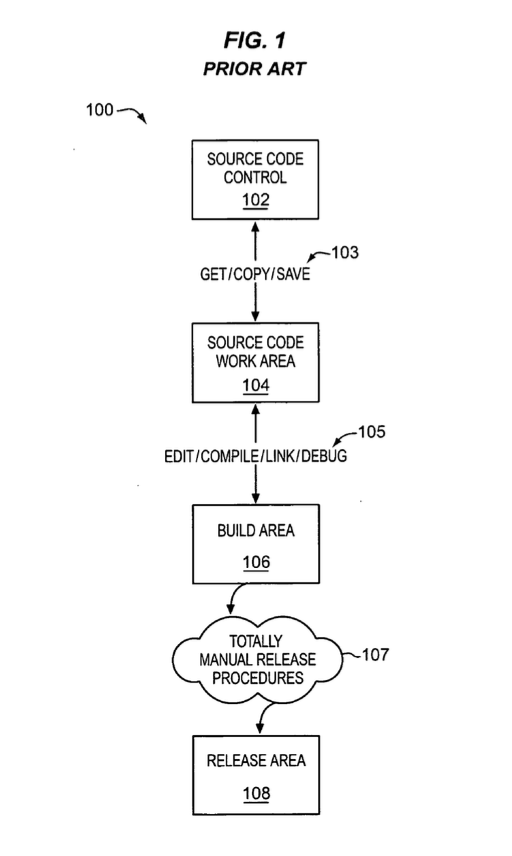
\includegraphics{/Users/kenzie/Documents/HoGent/Bachelorproef/Images/SRM_P_Fig1.png}
    \caption{Figuur uit \autocite{Barshefsky2005}. Flowchart van een niet geautomatiseerde versie beheer procedure.}
    \label{fig:FL_fig1}
\end{figure}
Het document \autocite{Barshefsky2005} beschrijft echter een aantal problematieken bij het idee uit figuur 1. Zo is dit een zeer manueel proces waarbij verschillende mensen deelnemen. Het is dus zeer gemakkelijk om fouten te maken tijdens een van deze stappen. Bijvoorbeeld een merge conflict. Deze hebben ze proberen te verhelpen door middel van computer geassisteerde release. Zie figuur 2. Ook is er in dit document nagedacht over de verschillende files en methodes om software te compileren en hoe deze beheerd moeten worden. Zo stellen ze gescheiden opslagplaatsen voor, voor inventory files en build files, enz. Zie figuur 3 voor details.
\newline
\newline
Dit document \autocite{Barshefsky2005} toont dus een nogal algemeen beeld over de software release cycli en wordt meer ter info beschouwd in dit onderzoek.
\newline
\newline
\subsection{Continuous Integration and Its Tools}
Bij release management hoort continuous integration en continuous development. Het volgende korte artikel \autocite{Meyer2014} bespreekt kort waarom een organisatie aan continuous integration moet doen en wat voor tools er allemaal bestaan. Ook worden er een aantal aanwijzingen gegeven rond het gebruik van continuous integration.
\newline
\newline
Het artikel \autocite{Meyer2014} vertrekt vanuit het stand punt dat een versie beheer tool in ieder softwarebedrijf een gegeven moet zijn. Dit om situaties te vermijden dat het lokaal werkt maar op andere toestellen niet. Ook staat dit toe om volledige geautomatiseerde pipelines te maken die automatisch de code gaat compileren en controleren op fouten door meegeleverde testen of door een uitrol te doen, in een test omgeving. Het artikel gaat verder met te stellen dat het bij iedere organisatie een prioriteit moet zijn om ten aller tijden de builds werkende te houden. Dit staat dan niet alleen toe dat er ten allertijden een uitrol kan gedaan worden van werkende code naar een test omgeving, maar ook dat er geen fouten of niet werkende code wordt gepusht door de ontwikkelaars. Het artikel beschrijft verder een aantal tools zoals onder andere Jenkins voor het automatisch uitrollen en testen van nieuwe software.
\newline
\newline
Dit artikel \autocite{Meyer2014} is minder belangrijk voor dit onderzoek maar toont wel het belang aan van een build pipeline en een goeie test omgeving voor code werkende te houden en de kwaliteit de behouden.
\newline
\newline
\subsection{DeVops}
Devops is de overkoepelende term van release management en continuous integration and continuous development. Het is de bedoeling om de verschillende softwareteams onderling te doen communiceren en samenwerken. Dit met doel om beter en sneller software uit te rollen. Het volgende artikel \autocite{Ebert2016} legt in meer detail Devops uit. De 2 luiken van Devops worden besproken alsook waarom Devops belangrijk is. Ook worden veel tools en technieken aangehaald.
\newline
\newline
Het artikel \autocite{Ebert2016} begint met uit te leggen wat Devops voor een organisatie kan betekenen. Het stelt dat Devops staat voor een betere samenwerking tussen ontwikkelen, kwaliteit, zekerheid en operaties. Het is lang niet zo dat Devops voor ieder softwareproject kan gebruikt worden, maar het wordt toch aangeraden. Ook vertrekt het artikel uit een gegeven dat er al softwareversie beheer in enige vorm aanwezig is.
\newline
\newline
Verder stelt het artikel \autocite{Ebert2016} dat er 2 facetten zijn bij Devops. Enerzijds de build kant van de software en anderzijds het deployment gedeelte van de software. Builden wordt volgens het artikel hoofdzakelijk op twee manieren gedaan. Aan de ene kant zijn er de traditionele build tools die meestal nog wat handmatig werk vereisen. Om in deze tools een build te doen moet er meestal een xml gemaakt worden met specifieke onderdelen. Dit kan nogal arbeidsintensief zijn. Langs de andere kant zijn er contiuous integration procedures. Hierbij wordt getracht om op ieder moment test bare werkende code te hebben. Deze tools zijn een stuk gemakkelijker om te gebruiken en zijn meestal cloud gebaseerd. Dit is omdat het de bedoeling is om op een zeer vlot en sneller tempo updates te kunnen uitrollen. Het artikel beschrijft een tabel~\textcite{Ebert2016} waarin een aantal tools met wat rand info beschreven staan.
\newline
\newline
Het artikel \autocite{Ebert2016} stelt dat meestal hierna de software getest moet worden zodanig dat kwaliteit kan worden gegarandeerd. Dit moet zo efficiënt en snel mogelijk gebeuren waardoor er dus nood is aan infrastructure as code. Herbruikbare code die snel kan worden uitgevoerd over meerdere platformen. Verschillende automatisatie tools worden door het artikel besproken. De meeste zijn simpel in gebruik en gebruiken yaml of xml voor de test omgevingen te definiëren. Het uitrollen van test omgevingen voor de software wordt meestal in de cloud gedaan of met virtuele machines. Dit is afhankelijk van wat de vereisten zijn van de organisatie. 
\newline
\newline
Ook bespreekt het artikel \autocite{Ebert2016} een van de nieuwere manieren om software te testen. Ze bespreken het gebruik van microservices in de cloud. Hoofdzakelijk bespreekt het artikel de producten van Amazon AWS. Deze zijn zeer gemakkelijk te automatiseren en gemakkelijk in gebruik.
\newline
\newline
Dit artikel \autocite{Ebert2016} is een meer waarde voor dit onderzoek omdat er een hele hoop tools, naast elkaar, kort besproken worden. De nadruk ligt niet op gebruiksvriendelijkheid maar eerder op wat de tools ondersteunen en of dat ze snel bruikbaar zijn voor Devops procedures. Dit artikel bevestigd dat er in de use case van dit onderzoek een nood is aan een goed gebouwde omgeving omdat kwaliteit een nummer een prioriteit geworden is.
\newline
\newline
\section{Amazon AWS}
\subsection{Performance Analysis of High Performance Computing Applications on the Amazon Web Services Cloud}
Dit onderzoek wil ook de cloud platformen en hun aanbod naast elkaar leggen. Ook wilt dit onderzoek vlug een idee krijgen hoe de verschillende datacenters van de cloud providers samengesteld zijn en hoe de verbindingen hiermee zijn. De volgende paper \autocite{Jackson2010}is een prestatie test van een Amazon aws datacenter.
\newline
\newline
De paper \autocite{Jackson2010} gebruikt synthetische wetenschappelijke testen om de prestatie van een aantal Amazon producten te testen. Een Amazon datacenter is wat raar samengesteld aangezien de eindgebruiker geen enkel idee op voorhand heeft over welke hardware hij toegewezen krijgt in het datacenter. Bovendien is Amazon benadeelt op vlak van connectiviteit omdat het niet directe lijnen heeft naar de datacenters zoals Microsoft met Azure. Belangrijk is dat alle testen uitgevoerd door de paper, uitgevoerd zijn in hetzelfde datacenter.
\newline
\newline
In deze paper \autocite{Jackson2010} testen de onderzoekers vooral of dat een Amazon datacenter geschikt zou zijn voor wetenschappelijk gebruik. Vandaar dat er vooral synthetische wetenschappelijke tools gebruikt worden. De tools zijn zorgvuldig geselecteerd zodanig dat de verschillende aspecten van een datacenter worden getest. Zowel de processor, als RAM, de harde schijven en ook de verbinding met de servers worden getest.
\newline
\newline
De paper \autocite{Jackson2010} concludeert dat de prestatie van de systemen wel goed is maar dat het afhankelijk is van welk merk CPU de gebruiker krijgt. Aangezien hier geen controle over is, is het moeilijk om voor dezen redenen Amazon voor rekenintensieve doeleinden aan te raden. Ook is vastgesteld dat de connectie met het datacenter een aanzienlijke limitatie is voor taken die zeer transactie intensief zijn.
\newline
\newline
Deze paper \autocite{Jackson2010} is niet zo zeer een meerwaarde voor dit onderzoek. Het artikel is redelijk verouderd en ondertussen is Amazon een van de grotere cloud platformen. Ook bespreekt deze paper niet zo goed de producten van Amazon. Ook is de use case die de paper beschrijft totaal verschillend van de use case die dit onderzoek gebruikt. 
\newline
\newline
\section{Microsoft Azure}
\subsection{Microsoft Azure and cloud computing}
Aangezien binnen de use case van dit onderzoek Microsoft Azure een grote rol speelt, is het belangrijk om een zeer goed idee te vromen van hoe die cloud platform in elkaar zit en wat de verschillende services en producten zijn. Daarom is het volgende hoofdstuk uit een boek \autocite{Copeland2015} redelijk informatief, zeker om ergens te starten.
\newline
\newline
Het eerste hoofdstuk uit het boek \autocite{Copeland2015} is vooral bedoelt als een eerste kennismaking met het Azure platform. Azure is eigenlijk ontstaan uit Microsoft hun office 365 aanbiedingen. Microsoft biedt een grote hoeveelheid aan applicaties aan als onder deel van dit pakket. Omdat die applicaties ergens moeten draaien, is Microsoft begonnen met het bouwen van datacenters om daar hun SaaS (Software as a Service) in te hosten. Al snel beseften ze dat er geld viel te verdienen met het aanbieden van remote services. Het duurde dan ook niet lang vooraleer Microsoft ook begon met IaaS (Infrastructure as a Service) aan te bieden. Dit was toen een unicum volgens het boek \autocite{Copeland2015}, Aangezien tot dan de meeste cloud platformen ontstaan zijn vanuit het verhuren van overschot aan computing power uit een mengelmoes van toestellen uit een bepaald datacenter. Dit was onder andere een van de conclusies van een verouderd artikel over Amazon aws \autocite{Jackson2010}. Bij Microsoft waren dat speciaal gebouwde datacenters met die services in gedachten. Ook hun PaaS (Platform as a service) wordt kort aangehaald door het boek \autocite{Copeland2015}.

\textbf{Voorbeelden van Azure Iaas:}
\begin{itemize}
    \item Azure virtual machines
    \item Azure virtual networks
    \item Azure virtual networks gateways
    \item Azure storage solutions
    \item ...
\end{itemize}
\textbf{Voorbeelden van Azure Paas:}
\begin{itemize}
    \item Azure SQL database
    \item Azure website
    \item Azure content delivery network
    \item Azure DeVops
    \item ...
\end{itemize}
Verder legt het boek  \autocite{Copeland2015} kort uit wat vanuit Azure gedaan wordt op vlak van privacy en wetgevingen. Dit is minder interessant voor dit onderzoek. Ook gaat het boek kort in op waarom gebruikers, It professionals voor Azure cloud of een ander cloud platform zouden moeten kiezen. Zo haalt het boek  \autocite{Copeland2015} aan dat een cloud platform weinig onderhoud inhoud, minder dan een lokale opstelling. Ook is de eindgebruiker niet verantwoordelijk voor de hardware. Hun datacenter zijn redundant. Dus er is eigenlijk vrij weinig downtime. Ook de aangeboden producten zijn vrij compleet en gemakkelijk onderhoudbaar.
\newline
\newline
Verder geeft het boek  \autocite{Copeland2015} een korte introductie in het Azure web portaal. Deze heeft dit onderzoek voor kennismaking doeleinden eens doorgelopen. Veel interessants is hier voor dit onderzoek niet uit te melden. Het hoofdstuk is dus een snelle kennismaking met Azure. Dit dient als een basis voor verder onderzoek. Zo gaan we in deze literatuurstudie nog wat dieper in op Azure DeVops en een kleine hands-on. Ook IaaS van Azure wordt nog wat meer uitgediept.
\newline
\newline
\subsection{Microsoft Azure Documentation}
Zoals eerder aangehaald in deze literatuurstudie, speelt Microsoft Azure een belangrijke rol binnen de use case van dit onderzoek. Het is het vertrek punt voor de vergelijkingen. In het kader van dit onderzoek, is de website van Azure eens uitgeplozen. Dit omdat er een beeld kan gevormd worden over welke Azure services interessant kunnen zijn. Het volgende is een kort verslag. Er worden twee service categorieën aangehaald. Deze zijn Iaas en PaaS (Infrastructure as a Services en Platform as a Service). Specifiek is er gekeken naar Azure virtual machine, Azure virtual networks, Azure virtual gateways en Azure DeVops. Het laatste is een samenvatting van een onlinecursus van een uur en informatie op Microsoft Docs.
\newline
\newline
In het kader van software release management en dan vooral de stap om de kwaliteit van software te controleren, is er gekeken of er misschien een mogelijkheid is om deze specifieke infrastructuur eventueel in de cloud te maken. Hiervoor is er een kort concept uitgewerkt. Dit concept beschrijft een hybride infrastructuur (verwijzing) waarbij eigenlijk alle niet use case specifieke toestellen in de cloud zitten. In theorie stond dit toe dat alle infrastructuur dan als code zou kunnen worden gedefinieerd.
\newline
\newline
Het aanbod qua mogelijkheden voor hardware om een virtuele machine aan te maken op Azure is enorm. Ook in tegenstelling tot de concurrenten wordt er zeer transparant omgesprongen met welke hardware er per optie beschikbaar gesteld wordt. De mogelijkhden verschillen enorm en zijn meestal voor specifieke doeleindes. Ook de prijzen schalen mede met de use cases. Zo zijn er specifieke opties voor machine learning. Of een optie voor machines met enorme hoeveelheden ram en CPU-kracht om met bepaalde databases overweg te kunnen. Ook de goedkopere basis opties zijn redelijk uitgebreid. Al deze opties worden door Azure onderverdeelt in categorieën die door middel van een letter worden aangeduid. Zie figuur~\ref{fig:Chart_Azure_tiers}.
\begin{figure}[H]
    \centering
    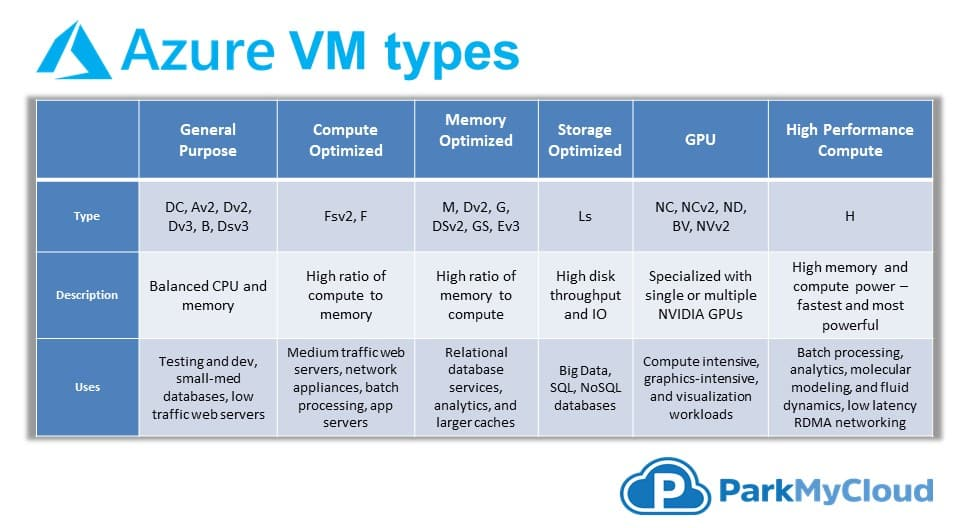
\includegraphics[width=\linewidth]{/Users/kenzie/Documents/HoGent/Bachelorproef/Images/azure-vm-types-comparison-1.jpg}
    \caption{Figuur van (https://p2zk82o7hr3yb6ge7gzxx4ki-wpengine.netdna-ssl.com/wp-content/uploads/azure-vm-types-comparison-1.jpg). Chart met alle VM tiers van azure en hun specifieke code.}
    \label{fig:Chart_Azure_tiers}
\end{figure}
Verder is Azure de oudere manier van het definiëren van een Azure virtual machine aan het afraden. Hiernaast zijn er ook nog een tal van mogelijkheden op vlak van virtual networking. Het belangrijkste is dat er een mogelijkheid bestaat om een virtueel netwerk volledig te isoleren van het internet. Dit staat toe dat enkel verkeer dat op dat specifieke netwerk is, aan de virtuele machines kan. Er wordt dan wel meestal een Azure network firewall node voorzien die in dit virtueel netwerk zit, zodanig dat de connectiviteit met de machines ten aller tijden gegarandeerd kan worden. Om dan connectiviteit te hebben met het virtueel netwerk wordt er gebruikgemaakt van een Azure Gateway node. Deze staat een point to point VPN (Virtual Private Network) tunnel toe. Dit is eigenlijk een directe, encrypteerde verbinding met het Azure netwerk. Hiervoor is wel specifieke hardware nodig lokaal in het netwerk. De kost van deze services is eigenlijk bijna niks. Azure werkt immers met een pay-to-run, pay-on-the-go system. Dit wil zeggen dat er dus moet betaald worden voor de aanmaak van de services en daarna voor het verbruik. Microsoft heeft op zijn documentatie portaal tal van stap voor stap handleiding voor het instellen van deze services. Ook concepten voor hybride opstellingen staan hier uitgelegd. Maar dit zou deze literatuurstudie te veel doen afwijken.
\newline
\newline
Het zou dus in theorie mogelijk moeten zijn om een hybride cloud infrastructuur te voorzien die dynamisch is voor de specifieke te testen projecten. De vraag is of dit handig is in gebruik en niet nodeloos complexiteit toevoegt.
\newline
\newline
Aure Devops in een platform van Azure dat organisaties toestaat om bepaalde procedures te definiëren voor het uitrollen van projecten. Het platform staat dan ook integratie toe met andere project follow-up tools van Microsoft. Deze procedures kunnen juist zoals de virtuele machines op Azure via code worden gedefinieerd of via een duidelijk en gemakkelijk te gebruiken GUI. De bedoeling van Azure DeVops is eigenlijk om het oude TFS-systeem te vervangen en een verbeterde interface aan te bieden. Meestal wordt DeVops gebruikt om aan Continuous Integration te doen. Dus er wordt een repository waar de code opstaat gedefinieerd. Hierna bestaat er een mogelijkheid om de code te compileren, automatisch testen te runnen en deze code dan weer door te schuiven naar een volgend stadium. Hier wordt de code dan uitgerold naar een omgeving voor verder kwaliteitscontrole. Het mooie aan dit platform is dat de gebruiker of organisatie niet verplicht is om deze code in een virtuele machine in de cloud te compileren of testen. Er is volledige controle over de procedures.
\newline
\newline
In het kader van dit onderzoek is dit zeer belangrijk aangezien dit platform op dit moment in gebruik genomen wordt. Er is ook een onlinecursus gevolgd met een basis uitleg en een labo. Dit heeft duidelijk gemaakt dat het mogelijk is om vanuit DeVops op een lokale test omgeving uit te rollen.
\newline
\newline